% Preamble ------------------------------------------------------------------------

\documentclass[11pt]{article}

 % Package Loads ------------------------------------------------------------------

 \usepackage[utf8]{inputenc}
 \usepackage[T1]{fontenc}
 \usepackage{lmodern}

 \usepackage[letterpaper, total={6.5in, 9in}, footnotesep=0.3in]{geometry}
 \usepackage[colorlinks=true, allcolors=blue]{hyperref}
 \usepackage{sidecap, caption}
 \usepackage{enumitem}
 \usepackage{csquotes}

 \usepackage{graphicx}
 \usepackage{float}

 \usepackage{units}
 \usepackage{amsmath,amsfonts,amssymb}
 \usepackage{gensymb}
 
 \usepackage{titlesec}
 \usepackage{titling}
 \usepackage{authblk}

 % Path ---------------------------------------------------------------------------

 \graphicspath{{assets/}}

 % Set Global Font ----------------------------------------------------------------

 \renewcommand{\rmdefault}{lmss}

 % Title Elements -----------------------------------------------------------------
 

 \title{
    {\vspace{-1.5cm}}
    {\hspace{-2cm}}   
    {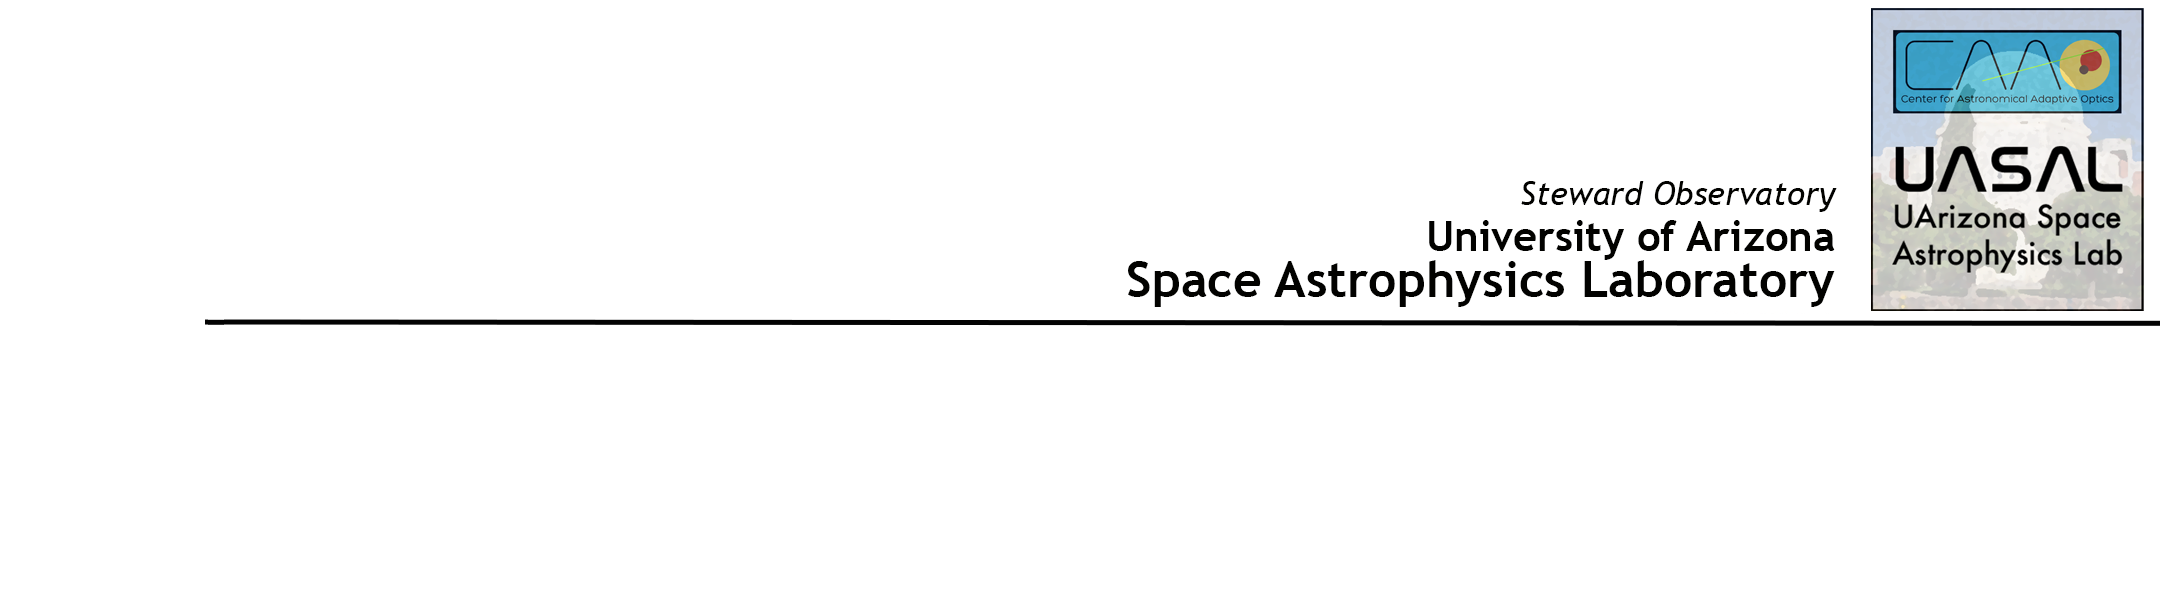
\includegraphics{assets/UASAL_Header.png}}
    {\large Preview of}\\
    {The SpaceX Starship}\\
    {\small \textit{General Consensus on Weights \& Fuel, and Calculated $\Delta$V}}
 } 

 \author{\large Jess Johnson}

 \affil{\small Senior Instrumentation Scientist \\ Steward Observatory, University of Arizona \\ July 2023}

 \date{}

% Document Start ------------------------------------------------------------------

\begin{document}

\fontfamily{lmss}
\maketitle

% Abstract ------------------------------------------------------------------------

\begin{abstract}

The following memo describes characteristics of the SpaceX Starship that may be important to the development of orbital trajectories. SpaceX has not released any finalized details on the vehicle's configuration as of this time, and a lot of the unofficial chatter on those details varies from week to week. What I have accumulated here is the general consensus on certain fundamental values that I have found in various reliable references, with those that have been repeated by more than one source given primacy. I have also provided basic $\Delta$V calculations based on those values, which can act as a rough comparison when considering orbits and other options.

\end{abstract}

\newpage

% Table of Contents ---------------------------------------------------------------

\tableofcontents
\newpage

% Section One ---------------------------------------------------------------------

\section{Description of the SpaceX Starship}
\subsection{Vehicle}

The Starship is the next heavy lifting space vehicle to be developed by Space X after the Falcon series. Like NASA's Space Launch System (SLS), the Starship system is meant to be a family of vehicle configurations that can be used to transport both human crews and space hardware, carry extra fuel to refuel other missions, and reach both earth orbit and interplanetary space. Unlike the SLS, however, the Starship is composed of mostly reusable parts, which reduces the cost of space access considerably.

The primary components are the Starship itself, consisting of a nose cone (configurable crew, cargo, and fuel transport), second stage booster engines, and fuel tanks; and the Super Heavy Booster, a gargantuan first stage booster that stands roughly 72m tall. When used together (as in Figure~\ref{fig:EntireStarship} below), the entire assembly is 122m from launch pad to tip of nose cone. It is the largest and most powerful rocket ever assembled, standing 10m taller than the Saturn 5 with more than twice the thrust.\cite{website:law21}

\begin{figure}[!b]
    \centering
    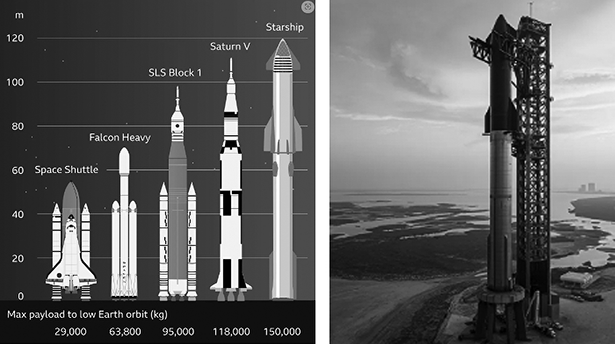
\includegraphics{assets/StarshipCompare.png}
    \caption{A comparison of spacecraft height and payload capacity, and a rendering of the Starship on its launchpad. (Images from BBC. Available at  https://www.bbc.com/news/science-environment-65334810)}
    \label{fig:EntireStarship}
\end{figure}

\subsection{Engines \& Fuel}
The Starship is powered by a new SpaceX engine, the 'Raptor'. The Raptor is a full-flow staged combustion cycle engine, meaning that it recycles the exhaust it uses to power its turbine into the combustion chamber where it is used a second time to directly produce thrust.\cite{website:wiki01} Figure~\ref{fig:RaptorSchematic} below is a simple schematic diagram of the Raptor engine. It burns the bi-propellent fuel Methalox, which, in the SpaceX formulation, is a combination of Liquid Oxygen and Liquid Methane at a 78:22 ratio.\cite{website:wiki01} Methalox is rarely used in spaceflight as Methane requires specific engine technologies to effectively ignite and burn, and SpaceX is the first to attempt a commercially usable design. 

The upper stage Starship will have six Raptors, three optimized for sea level and three optimized for vacuum (the Vacuum Raptor), providing a total of $1.47x10^7$ Newtons of thrust at maximum.  The Super Heavy Lifter will have a baseline of 33 Raptor engines, which can be increased or decreased as needed. This combination of engines provides a total of $7.45x10^7$ Newtons (maximum) of additional thrust.\cite{website:wiki01}

\begin{figure}[H]
    \centering
    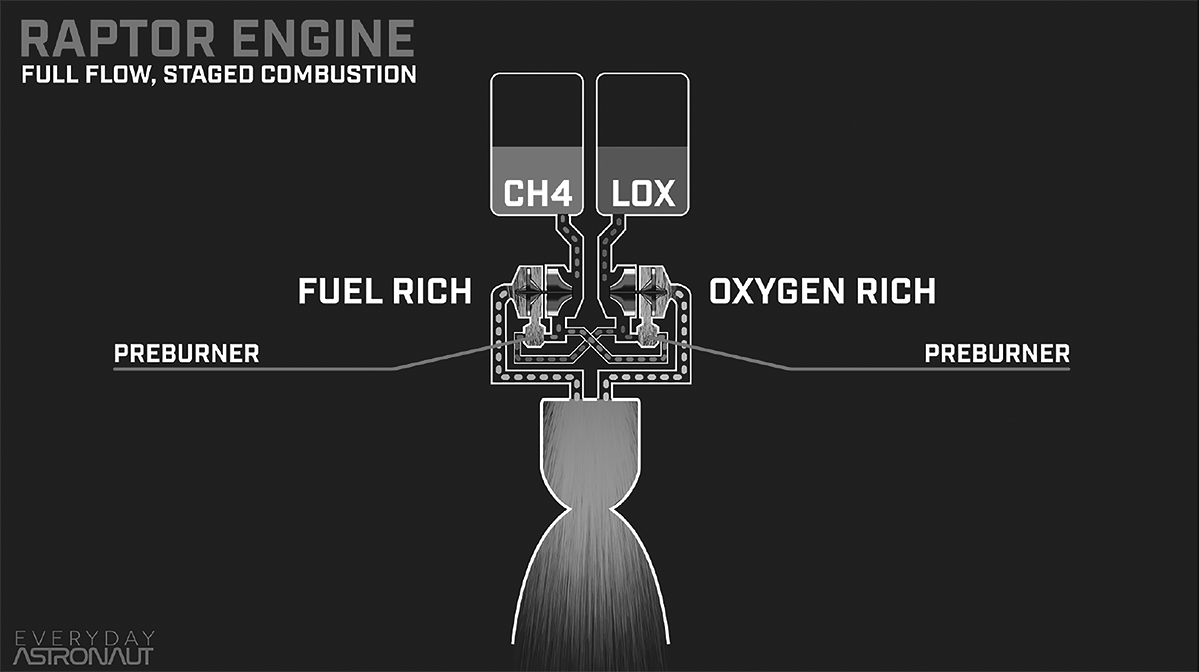
\includegraphics{assets/RaptorSchematic.png}
    \caption{Functional Schematic of the SpaceX Raptor Engine}
    \label{fig:RaptorSchematic}
\end{figure}

% Section Two ---------------------------------------------------------------------

\section{Payload}
\subsection{Fairing}

The standard Starship payload fairing is a clam shell structure 9m in outer diameter with an 8m dynamic envelope. Payload integration is accomplished by a mission-unique payload adaptor, which is also responsible for payload separation at time of deployment.\cite{spacex01}

The standard payload height is given as 17.24 m, but an extended payload height of 20m is also available. The payload profile is cylindrical, but tapered at the top, as shown in Figure~\ref{fig:StarshipPayload} (Diagram based on SpaceX illustration. SpaceX can mount NASA Shuttle style trunnion support system components along the sidewalls or the nose to provide structural support to the payload.\cite{spacex01} 

\begin{figure}[!b]
    \centering
    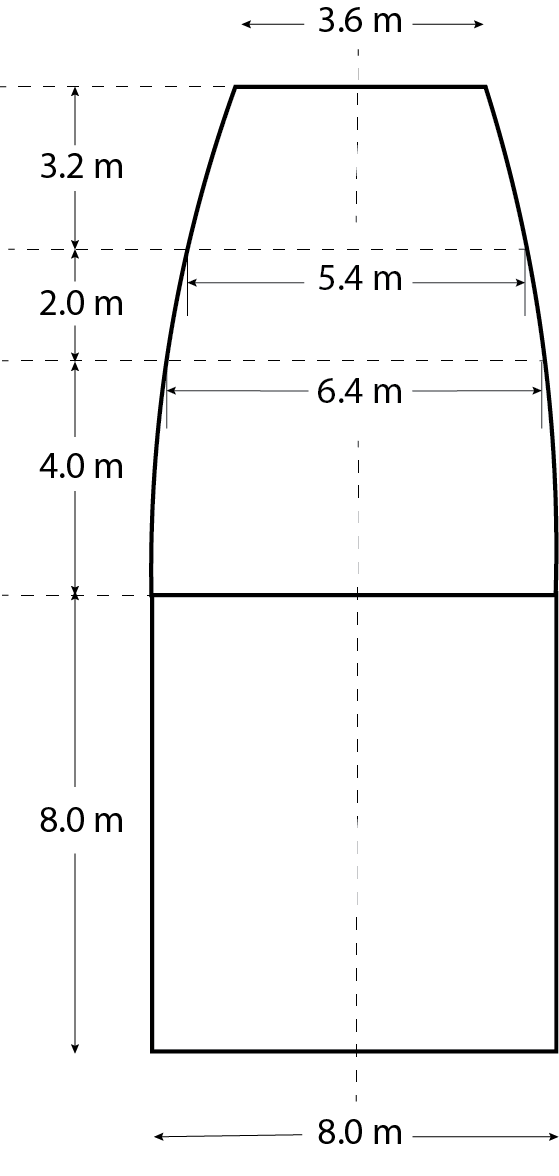
\includegraphics[height=3.5in]{assets/PayloadProfile.png}
    \caption{Vertical profile of Starship payload envelope.}
    \label{fig:StarshipPayload}
\end{figure}
\subsection{Payload Adaptor}

The Payload Adaptor is the physical structure used to connect the launch vehicle to the payload. It typically provides the electrical and data interfaces to the payload. SpaceX provides a payload adaptor that connects to 'standard payload interface systems' with a clampband separation system, or will integrate a custom adaptor provided by the client.

Standardized payload and power interfaces are provided, or electrical ground support equipment can be provided by the client. These interfaces are primarily provided for pre-launch monitoring and events, but some SpaceX interface functionality my be available in-flight.\cite{spacex01}

\subsection{Payload Environment}
SpaceX states that Starship's payload environment will "...meet or improve upon those of the Falcon Heavy Launch System", so an understanding of the Falcon's payload environment provides a baseline for specifications not yet provided for the Starship. The configuration used here is a Falcon Heavy with a 'standard' payload of 1,810 kg or more.

\subsubsection{Load \& Acceleration}
During launch and flight, a payload will experience a range of accelerations, both axially and laterally. Axial accelerations result from engine thrust and air drag; lateral accelerations result from first stage shutdown, wind gusts, and maneuvering by engine gimbal. Acceleration limits can be achieved by throttling the vehicle's engines, possible both on the Starship itself and the Super Heavy stage.

\begin{figure}[!b]
    \centering
    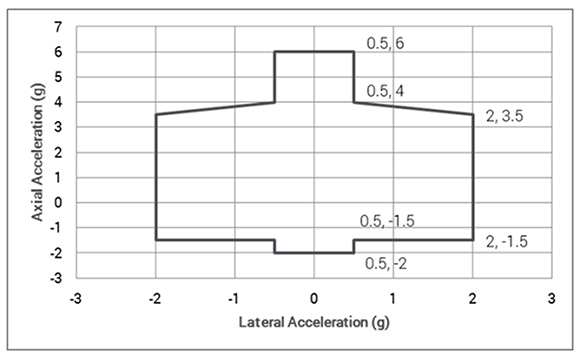
\includegraphics[height=2.25in]{assets/PayloadLoadMax.png}
    \caption{Graph of payload maximum design load factors. Diagram from SpaceX.}
    \label{fig:PayloadLoads}
\end{figure}

\begin{figure}[!t]
    \centering
    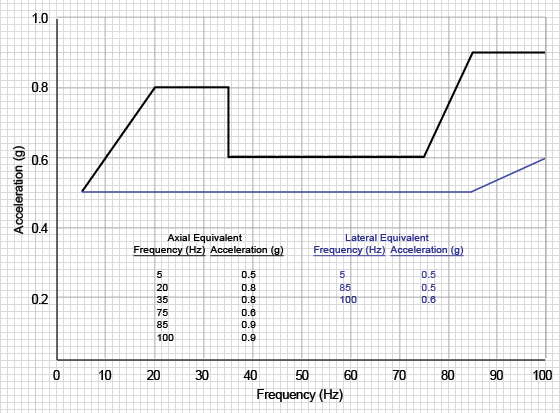
\includegraphics[height=2.5in]{assets/SineVibration.png}
    \caption{Graph of maximum sine vibration for the Falcon Heavy.  Axial equivalent vibration is in black; lateral equivalent vibration is in blue. Diagram from SpaceX.}
    \label{fig:SineVibration}
\end{figure}

Payload load factors are dependent on the dynamic coupling between vehicle and payload, but SpaceX has provided maximum expected design load factors for Starship. They are expressed in the plot shown in Figure~\ref{fig:PayloadLoads} below.\cite{spacex01} Lateral acceleration values are always positive. Positive axial values indicate compression; negative values indicate tension.\cite{bellini14}

\subsubsection{Sine Vibration}

SpaceX has not released information on maximum predicted sine vibration values for Starship, but they are available for the Falcon Heavy. Maximum levels are given for the top of the payload attachment fitting for an amplification level of Q=20 through Q=50, and are applicable at all stages of flight. (For a discussion of amplification factors and damping, see Irvine, 2005.\cite{website:irvine05} The limits are shown in Figure~\ref{fig:SineVibration} above.\cite{spacex01}

\subsubsection{Acoustic Environment}
Payloads are subjugated to a range of acoustic noise, originating from a variety of sources (engine noise resulting from the exhaust stream mixing with the atmosphere, atmospheric noise, aerodynamic excitation, etc.). The total acoustic energy being generated at any particular point is called the 'acoustic load'. Acoustic load levels are highest during liftoff and transonic flight. Lower frequencies contribute the majority of acoustic energy. The primary result of acoustic load is vibration.\cite{shakir09}

\begin{figure}[!b]
    \centering
    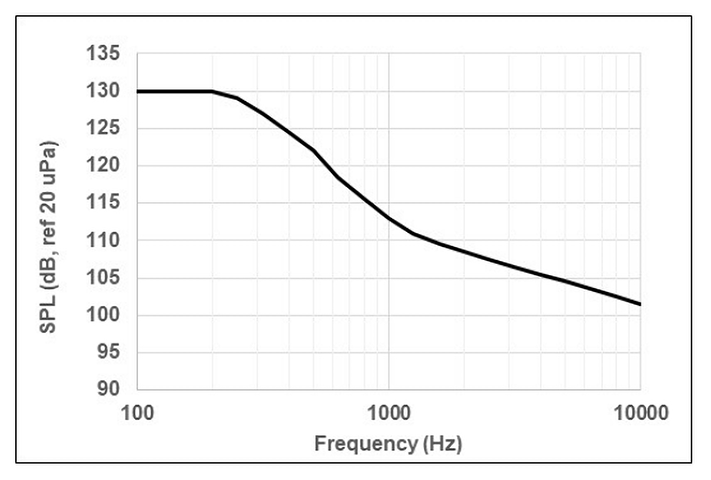
\includegraphics{assets/AcousticLevels.png}
    \caption{Graph of maximum predicted acoustic environmental levels. Diagram from SpaceX.}
    \label{fig:AcousticLevels}
\end{figure}

SpaceX has released limited information on the predicted acoustic load environment of the Starship. The maximum predicted acoustic environment levels in 1/3 octave bands are shown in the plot in Figure~\ref{fig:AcousticLevels} below.

\section{Mass \& Capacities}

Starship is large, in both size and weight. The following is not official, but culled from several sources.

% Section Three -------------------------------------------------------------------

\subsection{Starship Specifications}

Mass and cargo capacities for the upper stage Starship:
\newline

\begin{table}[H]
\begin{center}
\caption{\label{StarshipMassSpecs02}Table of Starship mass and cargo capacities.}
\begin{tabular}{||c c c c||} 
 \hline
 Description & Condition & Value & Units \\ [0.5ex]
 \hline\hline
 Starship Mass & Unloaded & 110 & Metric Tons \\ 
 \hline
 Starship Cargo Mass & Maximum & 120 & Metric Tons \\
 \hline
 Fuel Mass & Maximum & 1200 & Metric Tons \\
 \hline
 Total Starship Mass & Maximum & 1430 & Metric Tons \\
 \hline
\end{tabular}
\end{center}
\end{table}

\subsection{Super Heavy Booster Specifications}

Mass and fuel capacities for the lower stage Super Heavy Booster: 


\begin{table}[H]
\begin{center}
\caption{\label{BoosterMassSpecs}Table of Booster mass and fuel mass.}
\begin{tabular}{||c c c c||} 
 \hline
 Description & Condition & Value & Units \\ [0.5ex]
 \hline\hline
 Booster Mass & Unloaded & 270 & Metric Tons \\ 
 \hline
 Fuel Mass & Maximum & 3300 & Metric Tons \\
 \hline
 Total Booster Mass & Maximum & 3570 & Metric Tons \\
 \hline
\end{tabular}
\end{center}
\end{table} 

Combined, this gives us the following Specifications for the full Starship configuration:
\newline

\begin{table}[H]
\begin{center}
\caption{\label{StarshipMassSpecs}Table of combined Starship and Booster mass and cargo capacities.}
\begin{tabular}{||c c c c||} 
 \hline
 Description & Condition & Value & Units \\ [0.5ex]
 \hline\hline
 Starship and Booster Mass & Unloaded & 380 & Metric Tons \\ 
 \hline
 Starship Cargo Mass & Maximum & 120 & Metric Tons \\
 \hline
 Fuel Mass & Maximum & 4500 & Metric Tons \\
 \hline
 Total Starship and Booster Mass & Maximum & 5000 & Metric Tons \\
 \hline
\end{tabular}
\end{center}
\end{table}

\subsection{Starship Fuel}

The Starship uses the bi-propellent fuel Methalox, composed of Liquid Oxygen and Liquid Methane. SpaceX Methalox is ($LCH_4$) in a 78:22 mass ratio. 

  The density of Liquid Oxygen at STP is $\rho_{{LO}_4}=1141 kg/m^3$, and the density of Liquid Methane at STP is $\rho_{{LCH}_4}=424 kg/m^3$.  The density of the combined liquids is then:


\[M_{comb}=78 kg + 22 kg=100 kg\]
\[V_{comb}=\frac{M_{{LO}_4}}{\rho_{{LO}_4}}+\frac{M_{{LCH}_4}}{\rho_{{LCH}_4}}=1.07x10^-1 \frac{kg}{m^3}\]
\[\rho_{Methalox}=\frac{100kg}{1.07x10^-1 \frac{kg}{m^3}}=933.1 \frac{kg}{m^3}\] 
\newline


In terms of metric tons, this is $\rho_{Methalox}=.9331 \frac{t}{m^3}$. The Starship's fuel capacities and weights are then: \newline

\begin{table}[H]
\begin{center}
\caption{\label{FuelSpecs}Table of fuel capacities and volumes.}
\begin{tabular}{||c c c c c||} 
 \hline
 Description & Condition & Value & Units & Notes \\ [0.5ex]
 \hline
 Starship Fuel Capacity & Loaded & 1200 & Metric Tons & (2,645,000 lbs) \\ 
 \hline
 Starship Fuel Volume & Loaded & 1286 & Cubic Meters & (45,415 Cubic Feet) \\
 \hline
 Booster Fuel Capacity & Loaded & 3300 & Metric Tons & (7,275,255 lbs) \\ 
 \hline
 Booster Fuel Volume & Loaded & 3537 & Cubic Meters & (124,908 Cubic Feet) \\
 \hline
 Total Combined Capacity & Maximum & 4500 & Metric Tons & (9,920,255 lbs \\
 \hline
 Total Combined Volume & Maximum & 4823 & Cubic Meters & (170,323 Cubic Feet) \\
 \hline
\end{tabular}
\end{center}
\end{table} 



% Section Four --------------------------------------------------------------------

\section{Delta V}

\subsection{The Rocket Formula}

The fundamental equation in rocket science is the Tsiolkovsky Rocket Equation. In a rocket powered by a reactive engine system, the engine system consume propellant, creating the force that moves the rocket while decreasing the rocket's overall mass. The decrease in mass is therefore related to the change in velocity:

\[\Delta V = v_e \cdot ln \left( \frac{m_0}{m_t} \right)\]

$v_e$ here is the \emph{exhaust gas velocity} as the gas leaves the exhaust cone. It is sometimes referred to as \emph{effective exhaust gas velocity}, indicating that it is the mean velocity over the exhaust cone's aperture. $m_0$ is the initial, fully loaded mass of the rocket. $m_t$ is the mass of the rocket after all fuel has been expended. 

For completeness, the rocket formula can also be expressed in terms of the \emph{Specific Impulse, $I_{SP}$}, of the engine. Specific Impulse is the engine's efficiency at generating thrust, and is the change of momentum produced per unit mass of fuel. Specific Impulse is a time... it is the time for which an engine can generate thrust equal to its mass in the earth's gravitational field (1g). The relationship between exhaust gas velocity and specifc impulse is:

\[v_e=I_{SP} \cdot g_0\]

Using this, it is possible to write the rocket equation in terms of specific impulse:

\[\Delta V = I_{SP} \cdot g_0 \cdot ln \left( \frac{m_0}{m_t} \right)\]

\subsection{Calculating \(\Delta V \)}
\subsubsection{Value for Methalox $v_e$}

The value of the exhaust gas velocity for a propulsive fuel is critical to calculate Delta V. We will calculate it from fundamentals, approaching it from specific impulse. This calculation gives the upper limit on exhaust velocity.

First, equate the kinetic energy of the exhaust gas to the chemical energy stored in the fuel:

\[E=\frac{1}{2} mv_e^2\]
\[v_e = \sqrt{\frac{2E}{M}}\]

Then:

\[\frac{\sqrt{\frac{2E}{M}}}{g}=\frac{v_e}{g}=I_{SP}\]

$\frac{E}{m}$ is chemical energy density, $\mu$. so we can restate specific impulse as:

\[I_{SP}=\frac{\sqrt{2 \mu}}{g}\] 

$\mu$ is the chemical energy in the Methalox reaction, which is:

\[CH_4^{(g)}+2O_2^{(g)} \rightarrow CO_2^{(g)}+2H_2O^{(g)}\]

A combustion table will, however, give the following reaction:

\[CH_4^{(g)}+2O_2^{(g)} \rightarrow CO_2^{(g)}+2H_2O^{(l)}\]

This is the \emph{enthaply change of combustion, $\Delta H$}. To get the correct answer, we have to factor in the  enthalpy change of
\[2H_2O^{(l)} \rightarrow 2O_2^{(g)}\]

which is just the heat of vaporization, $\Delta H_{vap}$. So $\mu$ becomes:

\[\mu=\frac{\Delta H-\Delta H_{vap}}{m_m}\]

and:
\[I_{SP}=\frac{\sqrt{\frac{2(\Delta H-\Delta H_{vap})}{m_m}}}{g}\]

We have to vaporize two moles of water for every mole of Methane we burn through, so:

\[\Delta H_{vap}=2 \cdot 40.2 \frac{kJ}{mol} = 80.4 \frac{kJ}{mol}\]  
\newline

The relevant molar masses are $44 \frac{g}{mol}$ for $CO_2$ and $18 \frac{g}{mol}$ for $H_2O$, so:

\[M_m=44+2\cdot18=80 \frac{g}{mol}\] 

From online sources, $\Delta H = 890.3 \frac{kJ}{mol}$. We know $g$, so plugging in gives us:

\[I_{SP} = 458.7 s\]

In terms of exhaust velocity:

\[v_e = I_{SP} \cdot g = 4500 \frac{m}{s}\]

\subsubsection{Starship Delta V Values}

With this value for the exhaust velocity and the above values for available fuel, we can calculate the total Delta V for the Starship in both configurations (with and without the Super Heavy Booster phase). These are shown in the following table.  
\newline

\begin{table}[H]
\begin{center}
\begin{tabular}{||c c c c c||} 
 \hline
 Configuration & Initial Mass & Final Mass & Ln of Ratio & Total $\Delta V$ \\ [0.5ex]
 \hline
 Starship Only & 1430 t & 230 t & 1.827 &  8,223 $\frac{m}{s}$  \\ 
 \hline
 Starship and Booster & 5000 & 500 & 2.303 & 10,362 $\frac{m}{s}$  \\
 \hline
 
\end{tabular}
\caption{\label{FuelSpecs02}Table of fuel capacities and volumes.}
\end{center}
\end{table} 

As a rule of thumb, Delta V to low earth orbit is roughly 7500 m/s. 

\newpage

% Bibliography --------------------------------------------------------------------

\bibliographystyle{plain}
\bibliography{bibliography}

\end{document}
